\documentclass[12pt]{article}
\usepackage[margin=1.0in]{geometry}
\usepackage{amsmath,amsthm,amssymb,amsfonts}
\usepackage{enumerate,mathtools}
\usepackage{pgfplots}
\usepackage{caption}
\usepackage{float}

\newtheorem{theorem}{Theorem}[section]
\graphicspath{ {./images/} }

\title{Shortest Path Algorithm:\\
Terminology and Theoretical Concepts}
\author{
Mark Wesley Harris
}
\date{\today}

\begin{document}
\maketitle

\section{Introduction}\label{sec:intro}
This document breifly explains the theoretical concepts behind the
Shortest Path Algorithm developed in this repository. This algorithm attempts
to solve the Traveling Salesman Problem, with the input of a 2D graph of datapoints
represented on a Cartesian coordinate system.

\section{Input Requirements}\label{sec:req}
There are some requirements that must be met by the input to this algorithm.
These are outlined below:
\begin{enumerate}
\item Data must be represented on a 2D Cartesian plane
\item The weights between vertices must be the distance between them
(i.e. the weight between pionts $p:(x_1, y_1)$ and $q:(x_2, y_2)$ is $\sqrt((x_1 - x_2)^2 + (y_1 - y_2)^2)$)
\end{enumerate}

\section{Definitions}\label{sec:def}
\begin{itemize}
\item $(x,y)$: the definition of a point with coordinates $(x,y)$.
\item $<p,q>$: the definition of a vector from point $p$ to point $q$.
\item $[s_1, s_2, ..., s_k]$: the definition for a path through a known set of edges.
\item $n$: the number of points in the dataset.
\item $\mathcal{V}$: the set of all vertices in the dataset.
Formally, $\mathcal{V} = \{p_1, p_2, ..., p_n\}$
\item $\mathcal{E}$: the set of all edges in the dataset.
The size of $\mathcal{E}$ is $n \times n$.
\item $\mathcal{H}$: the convex hull of the dataset.
Formally, $\mathcal{H} = \{h_1, h_2, ..., h_k\}$, where $k \leq n - 1$.
Given any set of points,
there is only one convex hull.
\item $\mathcal{S}$: the shortest path of a dataset as the set
$\mathcal{S} = \{s_1, s_2, ..., s_n\}$
of edges which are contained in the shortest path.
\item $\mathcal{E}'$: the set of all edges in the dataset that are in $\mathcal{E}$
but not $\mathcal{S}$.
Formally, $\mathcal{E}' = \mathcal{E} - \mathcal{S}$.
\item $\mathcal{W}$: the set of edges produced by the construction phase of the algorithm.
Formally, $\mathcal{W} = \{w_1, w_2, ..., w_m\}$, where $3 < m < n^2$.
\item $\mathcal{S}' \equiv \mathcal{S}$: the path $\mathcal{S}'$ has the same
perimeter as path $\mathcal{S}$
(they may or may not have the same edges).
\end{itemize}

\section{Theoretical Concepts}\label{sec:theory}
My algorithm is based upon many theoretical concepts I have discovered through
research and experimentation. They are explained below in different sections.

\subsection{Properties of Shortest Paths}\label{subsec:props}
I begin by describing the properties I have found to be true for all shortest
paths. These properties have been used to create the foundations for my algorithm.
\begin{enumerate}
\item For any two edges $s_i,s_j \in \mathcal{S}$ where
$i \neq j$, $s_i$ and $s_j$ do not cross. 
\item For any two edges $s_i,s_j \in \mathcal{S}$ where
$i \neq j$, $s_i$ and $s_j$ do not overlap. 
\item No edge $s \in \mathcal{S}$ intersects a point
$p \in \mathcal{V}$ where $s_1,s_2 \neq p$.
I.e. if an edge $e$ intersects a point $p$ that isn't an end point of $e$,
then $e \notin \mathcal{S}$.
\item If we were to add an arbitrary point $p_{n+1}$ to $\mathcal{V}$, $\mathcal{S}$
will not change iff $p_{n+1}$ is a point on the line of any $s \in \mathcal{S}$.
\end{enumerate}

\subsection{Invalidating a Segment}\label{subsec:invalid}
My algorithm is based upon the concept of invalidating as many segments of $\mathcal{E}$
as possible, but keeping all segments which could be in $\mathcal{S}$.
In order to do this,
I propose a method of construction that invalidates segments based upon the
properties for shortest paths which I have produced
above. Any segment which fails these properties cannot be in $\mathcal{S}$,
and so it should
not be included in $\mathcal{W}$.
\\\\
We test each line segment $w \in \mathcal{E}$ such that there is no point
$v \in \mathcal{V}$
where $v \neq w_1,w_2$ that lies on $w$.

\subsection*{Bijection Range Method}\label{subsec*:bijection-range-method}
...

\subsection*{Using Intersections}\label{subsec*:intersection-method}
The Bijection Range Method works for determining ranges on a segment $w$
for which points $p,q \in \mathcal{V}$ are closer to $w$ than $w_1$ or $w_2$.
However, since we are only interested
in invalidating the line with respect to this property, it is worth looking at
the possibility of using the intersection of any $e \in \mathcal{E}$ instead.
\begin{theorem}\label{thm:overlap}
For each $p,q \in \mathcal{V}$ where $p \neq w_1,w_2$ and $q \neq w_1,w_2$,
if $p$ and $q$ have overlapping Bijection Ranges
then the line passing through them intersects $w$.
\end{theorem}
\begin{proof}
The proof is shown below:
\begin{enumerate}[(1)]
\item Given that $p$ and $q$ have overlapping Bijection Ranges,
it is evident that there are 2 intersection points formed by
the lower and upper bounds of the intersection of ranges.
Let these points be $w_l$ and $w_u$.
\item By definition, these points form a quadralateral.
Let the quadralateral $p,w_l,q,w_u$ be denoted as $Q$.
\item Since $Q$ is a quadralateral,
a line segment can be drawn between $p$ and $q$ that lies within
the inner region formed by $Q$.
Let that line be denoted as $e$.
\item Since $w_l$ and $w_u$ both intersect $w$, and $e$ is a continuous line
that lies between $w_l$ and $w_u$, then $e$ must also intersect $w$.
\end{enumerate}
\end{proof}

\subsection*{Abstracting Bijection Ranges}\label{subsec*:bijection-range-method}
Calculating both bijections of each possible point $v \in \mathcal{V}$
for each edge $e \in \mathcal{E}$
is a very costly method of validating a segment. Instead of having to do the calculations
each time, it would be nice if there were a mathematical area to represent
when a point's bijection ranges will overlap for a given segment.
\begin{theorem}\label{thm:semicircle}
The area in which there is a bijection range created from point $p \in \mathcal{V}$
using segment $w \in \mathcal{E}$
can be represented as a semicircle, $M$, where $w$ is the segment opposite its arc.
\end{theorem}
\begin{proof} The proof is shown below:
\begin{enumerate}[(1)]
\item Let $w$ be the edge we are testing, with points $w_1,w_2 \in \mathcal{V}$.
\item Take a point $p \in \mathcal{V}$ where $p \neq w_1,w_2$ and $p$ does not lie on $w$.
\item Let $M$ be the unique semicircle in the direction of $p$ formed using $w$ as the
flat segment of $M$.
\item Let $A$, $B$, and $C$ represent the points $w_1$, $p$, and $w_2$, respectively.
Similarly, let $D$, $E$, and $F$ represent the midpoints of segments
$AC$, $BC$, and $AC$, respectively.
\item Now we assume the 3 cases for the position of $p$ relative to $M$:
\begin{enumerate}[(i)]
\item Assume that $p$ lies on the arc of semicircle $M$:
\begin{enumerate}[(a)]
\item Points $A$, $B$, and $C$ satsify the requirements of Thale's Theorem:
``if segment $AB$ is a diameter, then the angle at $C$ is a right angle.''
Thus $\angle ACB = 90$.
\item Let vector $V$ be the bijection of $BC$, so that $V$ passes through
$E$ and is perpendicular to $BC$.
Let the intersection point of $V$ and $AC$ be point $I$.
\item Since $\angle ABC$ = $\angle IBE$ and $\angle BCA = \angle BEI$,
$\triangle ABC$ and $\triangle IBE$ are similar triangles.
\item Given that $BE$ is half the length of $BC$,
then $BI = \frac{BA}{2} = BD$.
Thus $I$ is halfway between $A$ and $B$, so $I \equiv D$.
\item Now let $V$ be the bijection of $AC$, so that $V$ passes through
$F$ and is perpendicular to $AC$.
Let the intersection point of $V$ and $AC$ be point $I$.
\item Since $\angle BAC$ = $\angle IAF$ and $\angle ACB = \angle AFI$,
$\triangle ABC$ and $\triangle AIF$ are similar triangles.
\item Given that $AF$ is half the length of $AC$,
then $AI = \frac{BA}{2} = AD$.
Thus $I$ is halfway between $A$ and $B$, so $I \equiv D$.
\item Since both bijections for $p$ meet in the center of $w$,
the Bijection Range is a single point.
\end{enumerate}
This shows that the Bijection Range for points along the arc of $M$ are equal to
the center $w$.
\item Now assume that $p$ lies inside the area of $M$ but not on the arc of $M$:
\begin{enumerate}[(a)]
\item As shown above, if $p$ is on the arc of $M$ then $\angle ACB = 90$.
Thus if $p$ is inside the arc, $\angle ACB < 90$ or $\angle ACB > 90$.
\item As $p$ approaches $w$, $\angle ACB$ approaches $180$. So $\angle ACB > 90$.
\item Since $\angle ACB > 90$,
the two bijection vectors will intersect somewhere below $w$,
opposite to $M$.
\item The area between the intersections of these vectors with $w$ is
the Bijection Range found previously through iteration.
\end{enumerate}
This shows that the Bijection Range for points inside the area of $M$ is equal to the
intersection of the bijection vectors with $w$.
\item Now assume the final case, that $p$ lies outside the area of $M$ but not on
the arc of $M$:
\begin{enumerate}[(a)]
\item If $p$ is outside of the arc, then $\angle ACB < 90$.
\item Since $\angle ACB < 90$,
the two bijection vectors will intersect somewhere in the region above $w$,
on the same side as $M$.
\item The area between the intersections of these vectors with $w$ is not
the Bijection Range, since the inequalities will not contain the same ranges.
\end{enumerate}
Thus the Bijection Range for points outside the area of $M$ is undefined.
\end{enumerate}
\item This shows that the only possible way a Bijection Range is formed by
point $p$ on segment $w$ is if $p$ is inside or on the arc of semicircle $M$.
\end{enumerate}
\end{proof}

\subsection*{Final Segment Invalidation}
I have decided to classify a segment $w$ as a part of $\mathcal{E}'$ instead of
$\mathcal{W}$ (i.e. as ``invalid'') in the following manner:
\begin{align*}
&\begin{aligned}
\mathcal{E}' &= \{e'\text{ }|\text{ }\exists\text{ }e \in \mathcal{E} \text{ where } e \neq e'
\text{ and } e_1,e_2 \text{ have overlapping}\\
&\qquad \text{Bijection Ranges on opposite sides of } e'\}
\end{aligned}
\end{align*}
This means that for each edge $e' \in \mathcal{E}'$ there are two points,
$p,q \in \mathcal{V}$ which lie inside opposite semicircles
(by Theorem \ref{thm:semicircle}) and intersect $e'$ through an edge $e \in \mathcal{E}$
(by Theorem \ref{thm:overlap}). Since $\mathcal{W} = \mathcal{E} - \mathcal{E}'$,
$\mathcal{W}$ therefore contains all segments which were not intersected by two
points that have overlapping Bijection Ranges.
The set $\mathcal{W}$ for a random set of datapoints
in $[-10, 10]$ is produced below. I have overlaid the actual shortest path,
$\mathcal{S}$, in transparent blue. Notice that there is once segment which
was proved to be invalid which actually belongs to a shortest path.
\begin{figure}[h!]
\begin{center}
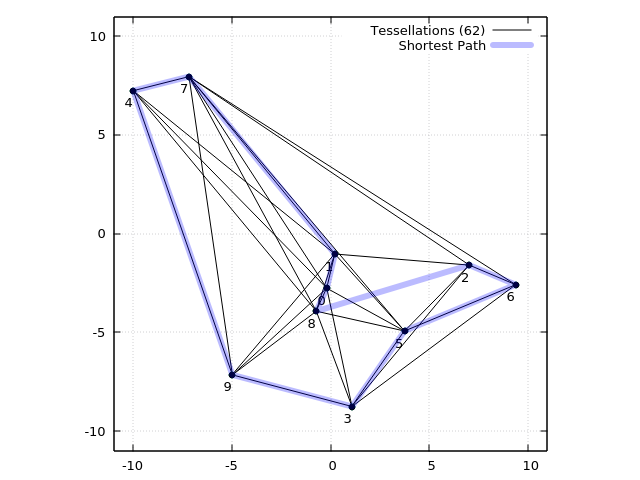
\includegraphics{w_random}
\end{center}
\caption{$\mathcal{W}$ And Actual Shortest Path}\label{fig:W-random}
\end{figure}
\\\\
There is another quality of $\mathcal{W}$ that we can notice by looking at many
outputs. While not all convex quadrilaterals in $\mathcal{W}$ have all possible segments
connected, it is clear from the instances where an edge $s$ is in $\mathcal{S}$ but
not in $\mathcal{W}$ that connecting the corners of each quadrilateral would...
\begin{figure}[h!]
\begin{center}
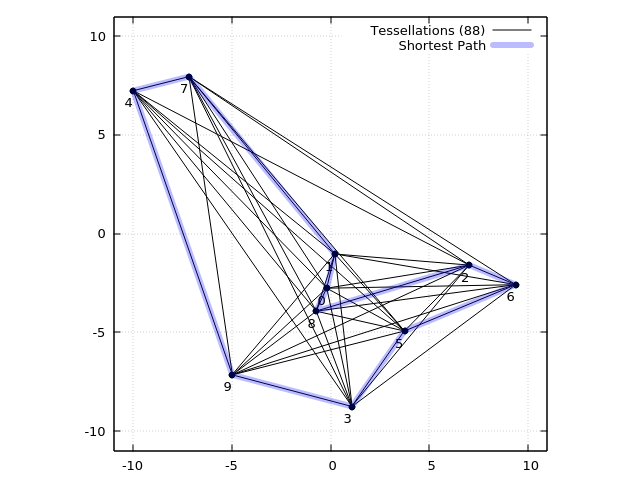
\includegraphics{w_quads}
\end{center}
\caption{$\mathcal{W}$ With Crossing Quadrilaterals}\label{fig:W-quads}
\end{figure}

\subsection{Expectations for $\mathcal{W}$}\label{subsec:exp_w}
Based upon the properites of shortest paths, $\mathcal{W}$ should have the following expectations:
\begin{enumerate}
\item $\mathcal{H}$ will always be included, since there are no paths
which could prove to invalidate any $h \in \mathcal{H}$.
\item Any two edges $w_i,w_j \in \mathcal{W}$ where $i \neq j$ can cross each other.
However any path $\mathcal{S}'$ can only contain one of these edges.
\item If an arbitrary point $p_{n+1}$ was added on an edge $w \in \mathcal{W}$,
$w$ would not be intersected by an edge $e \in \mathcal{E}$ where $e \neq w$.
\\\\
Derived from the construction phase of the algorithm,
$\nexists$ $w \in \mathcal{W}$ such that $w \in \mathcal{E}'$
given that $\mathcal{E}'$ is defined in the following way:
\begin{align*}
&\begin{aligned}
\mathcal{E}' &= \{e'\text{ }|\text{ }\exists\text{ }e \in \mathcal{E} \text{ where } e \neq e'
\text{ and } e_1,e_2 \text{ have overlapping}\\
&\qquad \text{Bijection Ranges on opposite sides of } e'\}
\end{aligned}
\end{align*}
Thus, if it were true that $p_{n+1} \in \mathcal{V}$,
the only path in $\mathcal{W}$ passing
through $p_{n + 1}$ would be the path $[w_1,p_{n+1},w_2]$.
All other paths have been proven to be invalid,
and thus unlikely to be part of the path $\mathcal{S}$.
\item A path $\mathcal{S}'$ can be made from $\mathcal{W}$
which goes through all vertices in $\mathcal{V}$ only once
and starts and ends on the same point.
If $\mathcal{W}$ has multiple paths that fit these requirements, then all such paths
$\{\mathcal{S}'_1, \mathcal{S}'_2, ... \mathcal{S}'_k\}$ should be collected.
The shortest path in this set is likely to be equivalent to $\mathcal{S}$.
\end{enumerate}

\section{The Algorithm}
The algorithm is made up of 3 consecutive phases,
Edge Invalidation, Path Generation, and Decision.
The Edge Invalidation Phase is
responsible for invalidating edges from $\mathcal{E}$ to generate the set
$\mathcal{W}$. The Path Generation Phase uses a greedy strategy to combine the resultant
shapes inside of $\mathcal{W}$ into a set of possible shortest paths,
$\mathcal{S}' = \mathcal{S}'_1, \mathcal{S}'_2, ... \mathcal{S}'_k\}$.
The Decision Phase chooses the shortest of these paths and returns it as the
found shortest path, $\mathcal{S}$.

\subsection{Edge Invalidation Phase}\label{subsec:edge-gen}
The goal of the construction phase of the algorithm is to generate $\mathcal{W}$,
i.e. a set of
edges $\mathcal{W} = \{w_1, w_2, ..., w_m\}$ such that
$\mathcal{W} \subseteq \mathcal{E}$ and $\mathcal{S} \subseteq \mathcal{W}$.
These edges must hold the properties of shortest paths, discussed in section
\ref{subsec:props}.
They must also give us some kind of meaningful information, so that we are able to
construct a path $\mathcal{S}'$ from them with the claim that
$\mathcal{S}' \equiv \mathcal{S}$.
The construction phase is broken up into steps below:
\begin{enumerate}
\item Choose an edge $e$ from $\mathcal{E}$ with the points $e_1,e_2$.
We will test this edge to see if it is possible that $e$ is part of a shortest path,
and subsequently that $e \in \mathcal{W}$.
\\\\
Take each edge $e' \in \mathcal{E}$ with points $p,q$ such that $p$ and $q$ straddle
$e$ and where $p$ is on the right side
of $e$ and $q$ is on the left side of $e$.
We perform the following tests to see if $e'$ invalidates $e \in \mathcal{W}$:
\begin{enumerate}
\item Let $V_1$ be the vector $<p,e_1>$.
\item Let $V_2$ be the vector $<p,e_2>$.
\item Find the bijection range of equality between $V_1,V_2$ and $e$,
represented as $r[lower, upper]$, as follows:
\begin{enumerate}
\item Let vector $B$ start from the bijection of $V_1$
in the direction of $e$ with length $|V_2|$.
\item Let the upper bound of $r$ be the intersection of $B$ and $e$.
\item Let $B$ start from the bijection of $V_2$
in the direction of $e$ with length $|V_1|$.
\item Let the lower bound of $r$ be the intersection of $B$ and $e$.
\end{enumerate}
\item Repeat steps (a) through (c) with $q$ instead of $p$.
\item If any of the intersections failed, $e'$ does not invalidate $e$,
so choose the next $e'$ and repeat from the beginning.
\item If all intersections suceeded, find the overall intersection area between
both $r$ ranges generated from steps (a) through (c) using $p$ and $q$.
\item If this intersection area is greater than the threshold, then $e$ is proven
invalid by $e'$. Choose the next $e$ and repeat from the beginning.
\end{enumerate}
\item If no $e'$ invalidated $e$, then $e \in \mathcal{W}$.
\end{enumerate}

\subsection{Path Generation Phase}\label{subsec:path-gen}
...

\subsection{Decision Phase}\label{subsec:decision}
...

\end{document}
